\section{Pipeline reliability: outer Generate$\rightarrow$Validate loop}
\label{app:reliability}

\S\ref{sec:pipeline} describes the outer
Generate$\rightarrow$Validate retry as a robustness mechanism
(up to three outer retries) but does not report how often it
fires in practice. To verify the loop does not silently rely on
retries, we re-ran SO-101 end-to-end with
\texttt{max\_outer\_gen\_val\_iters=3} and recorded the
per-phase outcome (Table~\ref{tab:reliability}). This rerun uses the spec-mode pipeline, whose
harness runs five tests; the self-contained onboarding harness
of \S\ref{sec:onboarding} runs seven per arm (Appendix~\ref{app:onboarding}).

\begin{table}[H]
\centering
\small
\begin{tabular}{lrr}
\toprule
\textbf{Phase} & \textbf{Status} & \textbf{Inner iterations used} \\
\midrule
01\_study     & OK & 4   \\
02\_generate  & OK & 7   \\
03\_validate  & OK & 5/5 tests pass \\
04\_export    & OK & N/A \\
05\_demo      & OK & N/A \\
\midrule
Outer iters used & \multicolumn{2}{l}{\textbf{1 of 3}} \\
Total wall-clock  & \multicolumn{2}{l}{\textbf{5.1\,min}} \\
Total LLM cost    & \multicolumn{2}{l}{\textbf{\$1.54}} \\
\bottomrule
\end{tabular}
\caption{SO-101 controlled rerun with outer retries enabled. The
inner Generate loop produces a driver that passes all five
structural tests on its first outer pass, so no
re-generation is triggered.}
\label{tab:reliability}
\end{table}

The interpretation is the one stated in \S\ref{sec:pipeline}: on
SO-101 the inner CodeAct loop within Generate is sufficient to
produce a passing driver; the outer retry exists as a safety
margin for harder embodiments rather than a frequently fired
recovery mechanism. We did not run a matching outer-retry sweep
on the other seven robots in the zoo; the headline 7.8\,min /
\$2.98 figures in \S\ref{sec:onboarding} use the same single
outer pass.

Figure~\ref{fig:pickbench} shows the pickbench scene used in
the \S\ref{sec:cap-cross-robot} end-to-end Pick experiment on
Piper, for which the synthesis pipeline was re-run against this
scene so the agent could synthesize the proximity-based grasp
routine itself.

\begin{figure}[H]
\centering
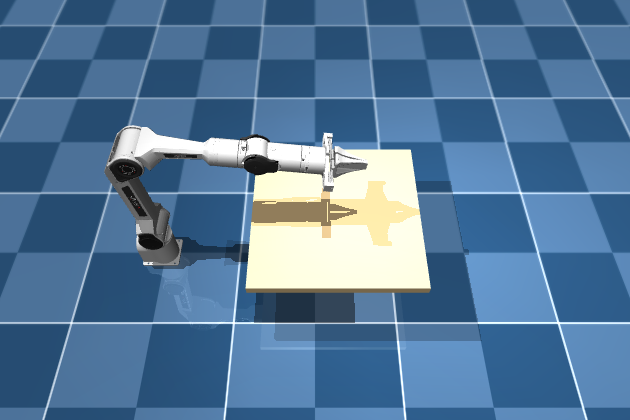
\includegraphics[width=0.85\columnwidth]{figures/pickbench_render.png}
\caption{The pickbench scene used for the Piper end-to-end Pick
experiment (\S\ref{sec:cap-cross-robot}). Three graspable cubes
(red, green, blue) sit on a 20\,cm $\times$ 20\,cm table within
Piper's reachable workspace.}
\label{fig:pickbench}
\end{figure}
